\documentclass[14pt]{article}

\usepackage[a4paper]{geometry}
\geometry{ hmargin=2.5cm, vmargin=1.5cm }

\usepackage{lmodern}
\usepackage{graphicx}
\usepackage{amsmath}
%\usepackage{placeins}
\usepackage{color}
\usepackage{alltt}

\usepackage[hyphens]{url}
\usepackage{blindtext}
 \usepackage{breakurl}
\usepackage[breaklinks=true]{hyperref}
%\usepackage[]{algorithm2e}
\usepackage{amssymb}
\usepackage{ulem}
\usepackage{subfig}
\usepackage{float}
\usepackage[english]{babel}
\usepackage[T1]{fontenc}  
\usepackage[utf8]{inputenc}
\usepackage{tcolorbox}
\usepackage{etoolbox}
\usepackage{minted}
\BeforeBeginEnvironment{minted}%
     {\begin{tcolorbox}}%
\AfterEndEnvironment{minted}
   {\end{tcolorbox}}%
\BeforeBeginEnvironment{inputminted}%
     {\begin{tcolorbox}}%
\AfterEndEnvironment{inputminted}
   {\end{tcolorbox}}%

\let\oldinputminted\inputminted
\renewcommand{\inputminted}[2]{\begin{tcolorbox}\oldinputminted[breaklines]{#1}{#2}\end{tcolorbox}}
  \setminted[python]{breaklines=true}
\let\oldhref\href
\renewcommand{\href}[2]{\oldhref{#1}{\detokenize{#2}}}


\setcounter{lofdepth}{1}
\setcounter{secnumdepth}{4}
\renewcommand{\thesection}{\Roman{section}}
\renewcommand{\thesubsection}{\thesection .\arabic{subsection}}
\usepackage{cite}
\renewcommand{\vec}[1]{\mathbf{#1}}



\newcommand{\R}{\mathbb{R}}
\newcommand{\Q}{\mathbb{Q}}
\newcommand{\C}{\mathbb{C}}
\newcommand{\Z}{\mathbb{Z}}
\renewcommand{\L}{\mathcal{L}}
\newcommand{\ltorle}{\overset{\scriptscriptstyle{<}}{\scriptscriptstyle{\le}}}
\newcommand{\diag}{\mathop{\mathrm{diag}}}
\newcommand{\ind}{\mathop{\mathrm{ind}}}




\title{Astro-archeology - Using NASA's data for space archeology}
\begin{document}

\date{}
\maketitle

\section*{Intro}

Back in 2015, NASA published this pretty earthrise picture as seen by the Lunar Reconnaissance Orbiter.
\begin{figure}[H]
  \centering
  \subfloat {\includegraphics[width=0.8\textwidth]{./data/lro_render_cropped_photoshopped.png}}
  \label{img:lro_render_tweaked_photoshop}
\end{figure}

Actually, I lied. Minus the cheating with the photoshopped earth from the original picture, this is a 100\% computer generated image.

Here is a gallery of recreated shots
\begin{figure}[H]
  \centering
  \subfloat [Original image captured by the spacecraft]{
    \includegraphics[width=0.3\textwidth]{./data/lro_earthrise_real.jpg}
  }
  \qquad
  \subfloat [Computer generated image of the scene]{
    \includegraphics[width=0.3\textwidth]{./data/lro_render_cropped.png}
  }
  \caption{LRO earthrise comparison, \href{https://www.nasa.gov/image-feature/goddard/lro-earthrise-2015}{post for the original} }

\end{figure}

\begin{figure}[H]
  \centering
  \subfloat [Original image captured by the spacecraft]{
    \includegraphics[width=0.3\textwidth]{./data/lro2_real_cropped.png}
  }
  \qquad
  \subfloat [Computer generated image of the scene]{
    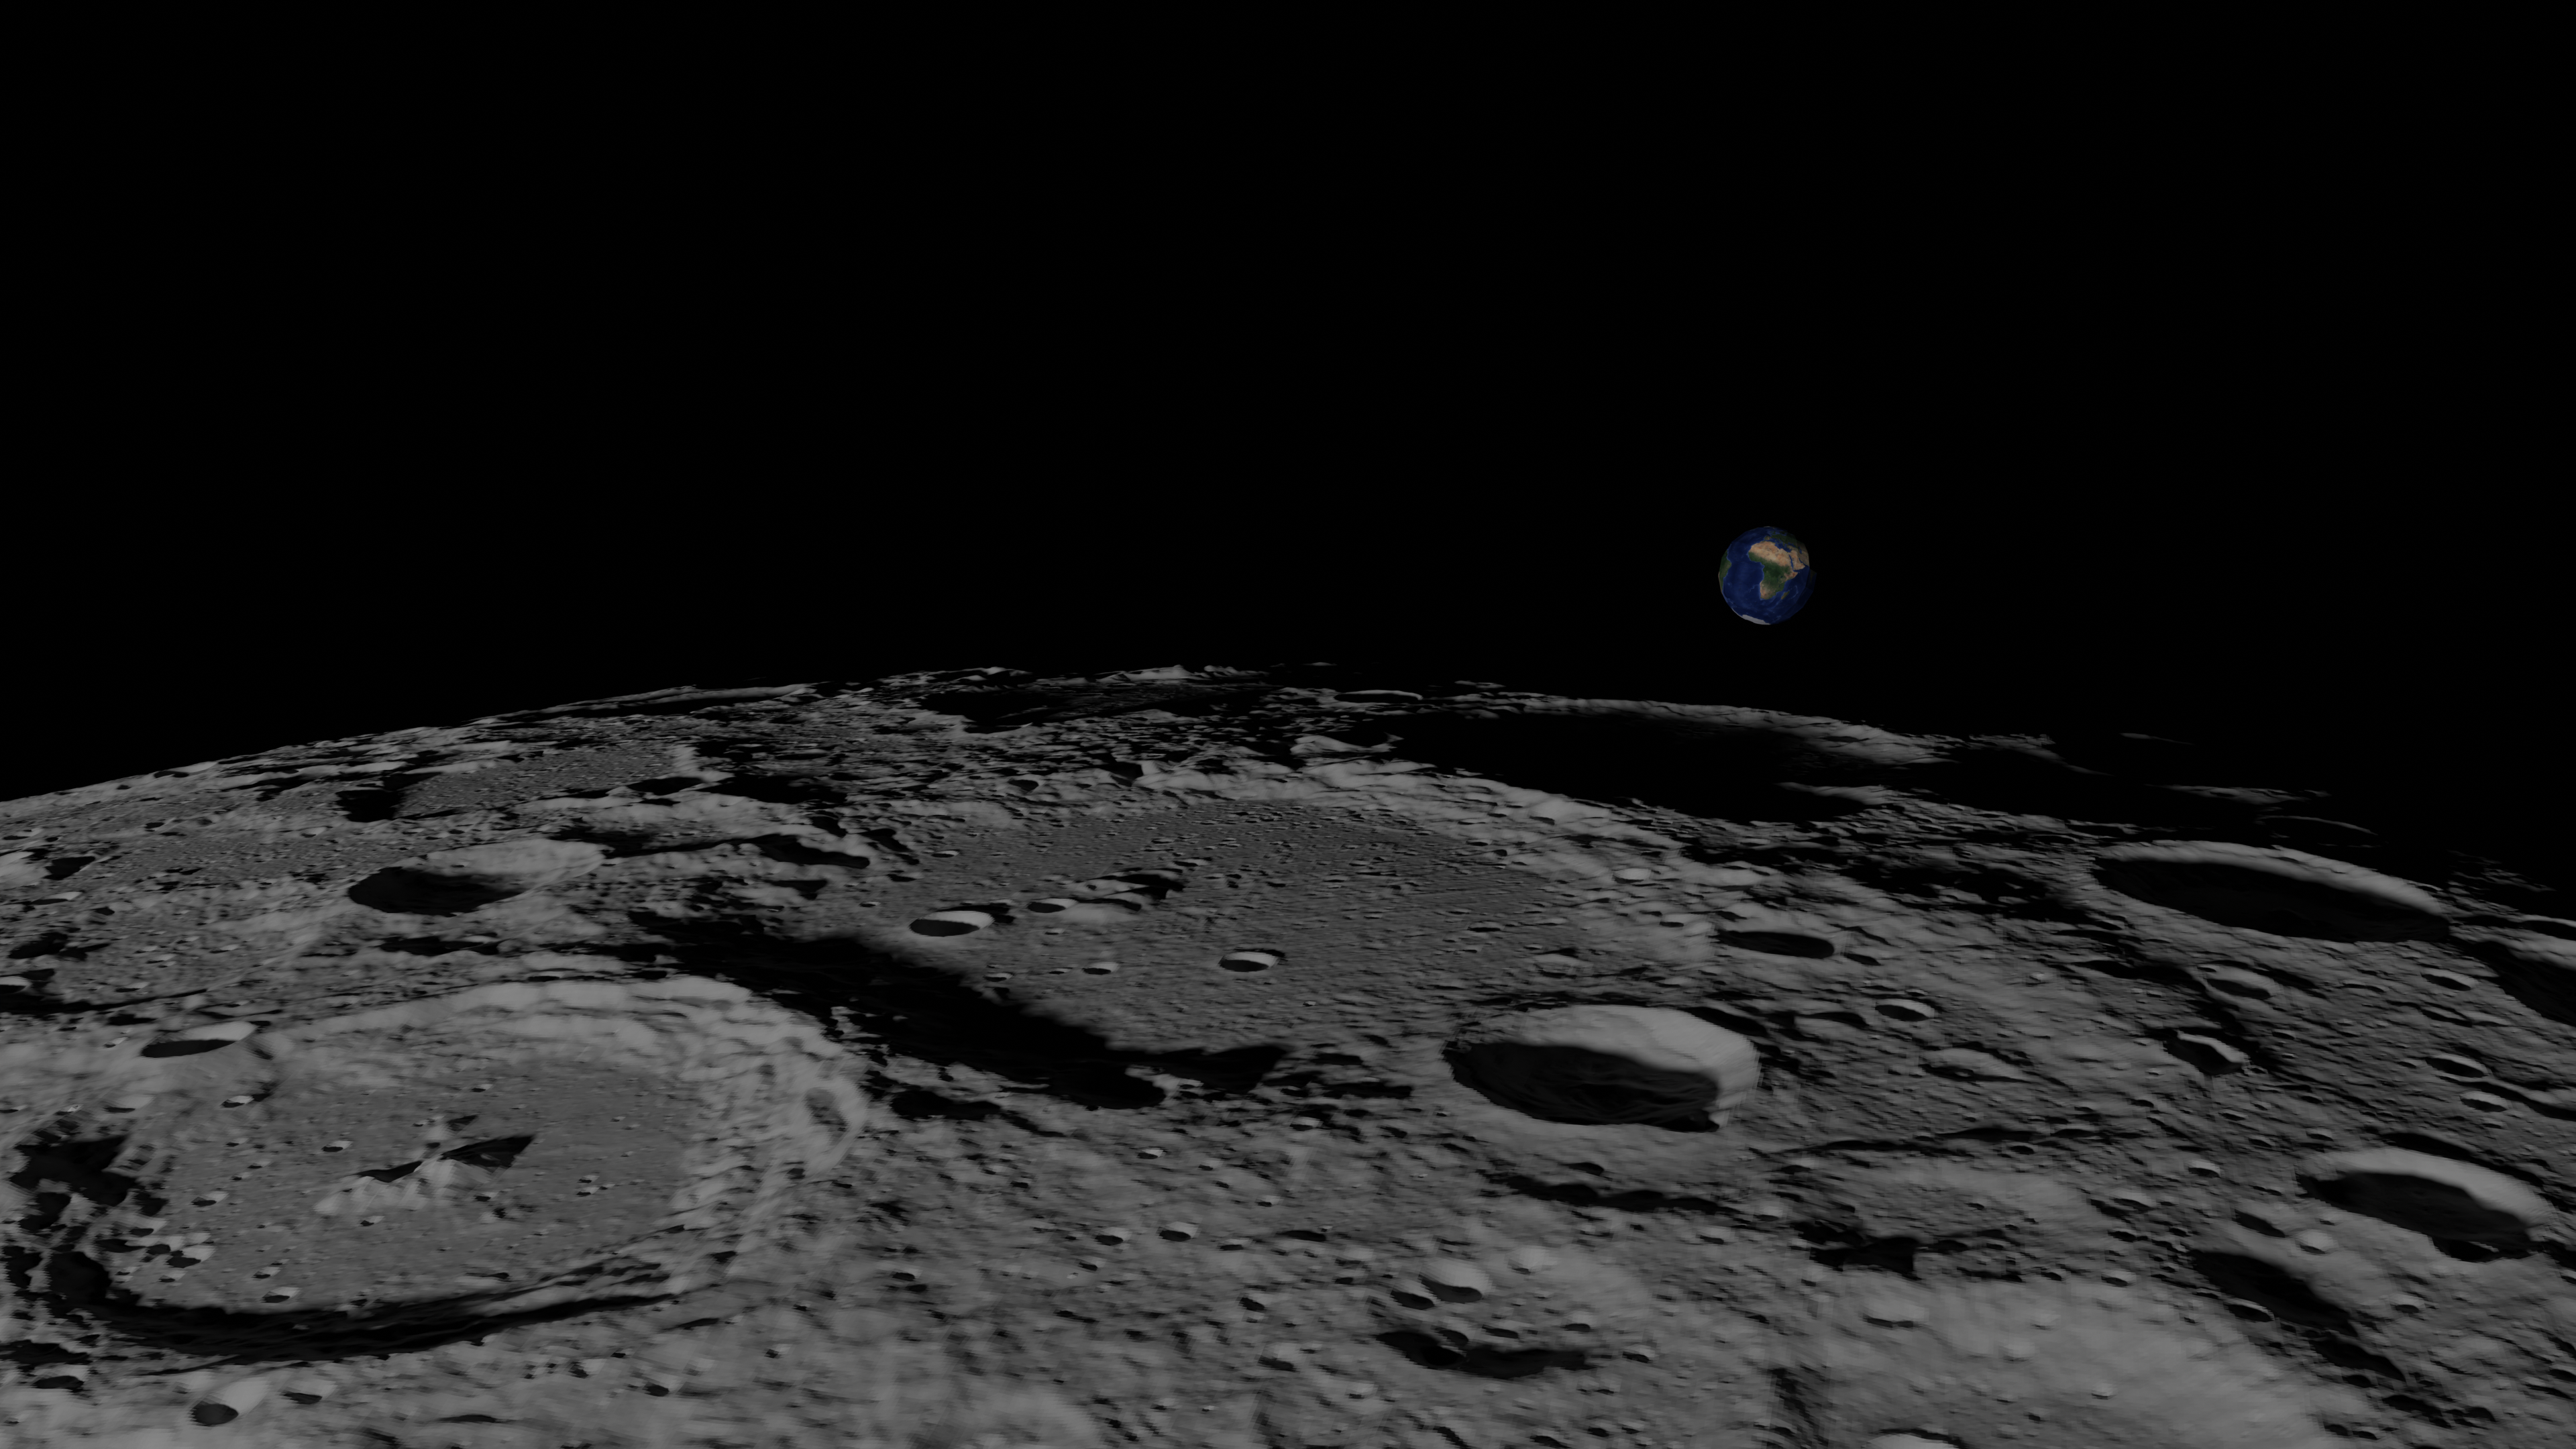
\includegraphics[width=0.3\textwidth]{./data/lro2_render.png}
    \label{img:lro_render_tweaked}
  }
  \caption{Another LRO earthrise comparison, this time at the pole, \href{http://lroc.sese.asu.edu/posts/764}{post for the original} }
\end{figure}

\begin{figure}[H]
  \centering
  \subfloat [Original image captured by the spacecraft]{
    \includegraphics[width=0.3\textwidth]{./data/kaguya_orig.jpg}
  }
  \qquad
  \subfloat [Computer generated image of the scene]{
    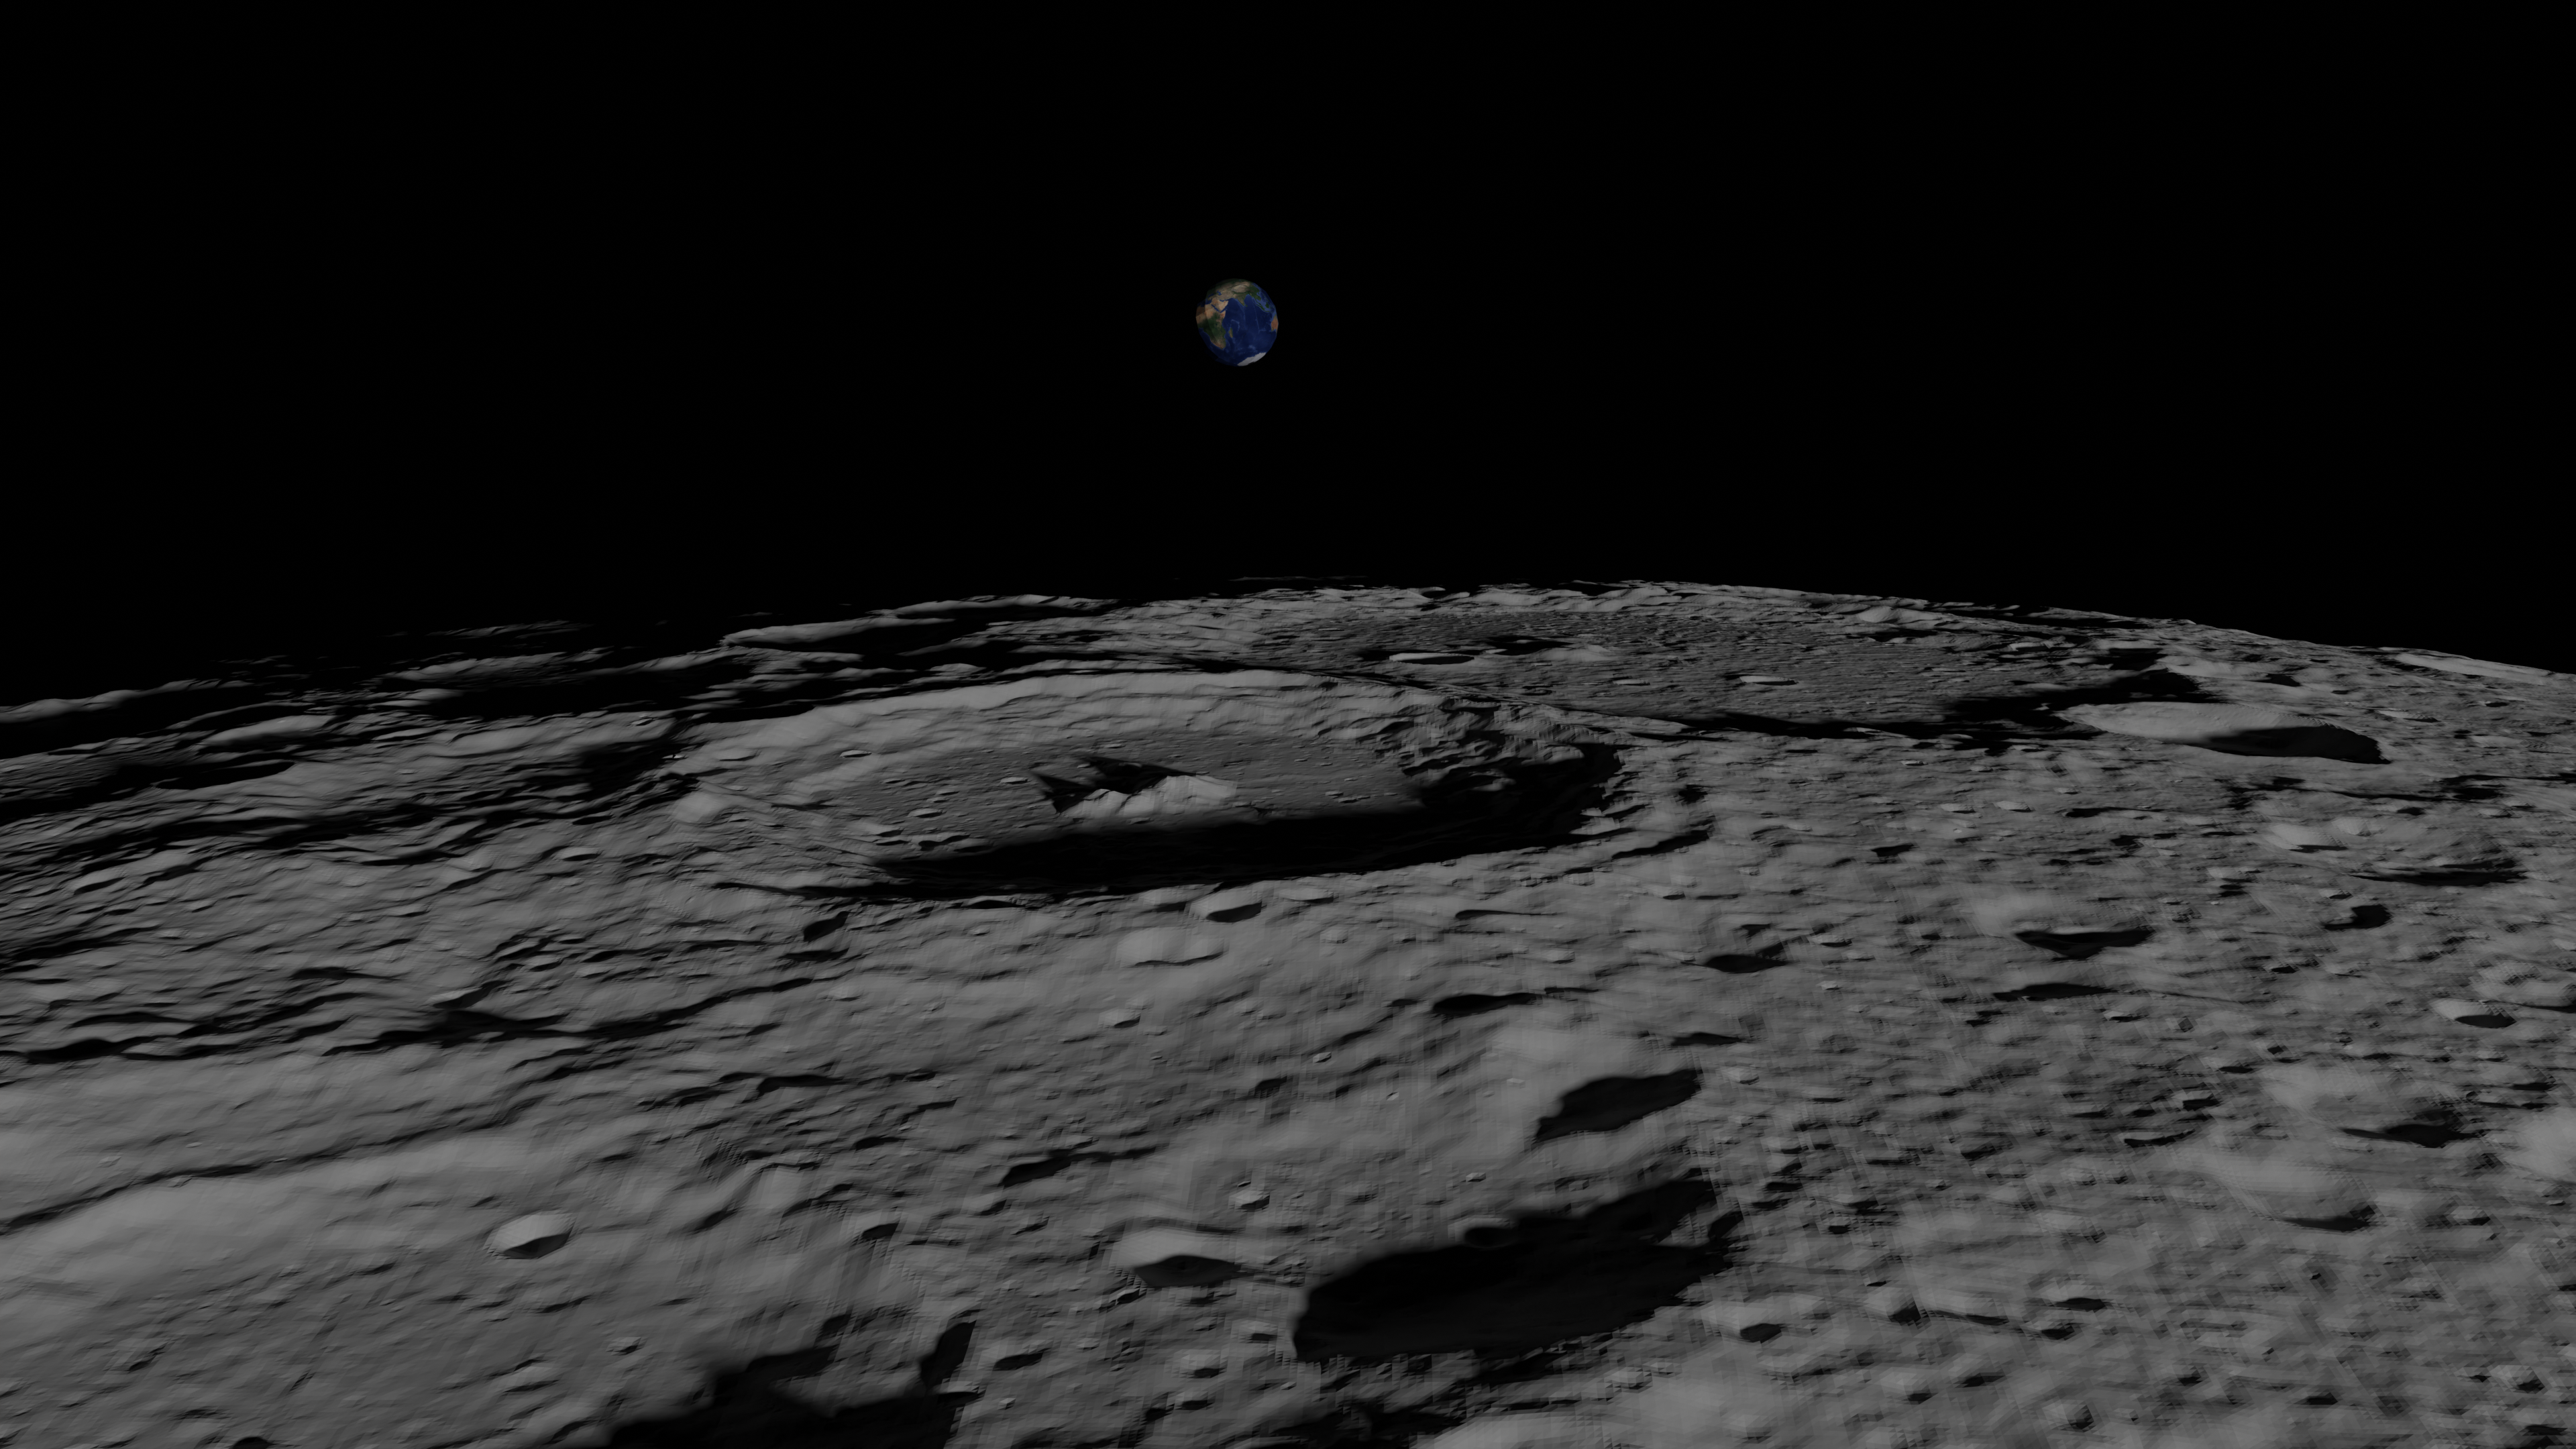
\includegraphics[width=0.3\textwidth]{./data/kaguya_render.png}
  }
  \caption{Kaguya earthrise comparison, \href{https://global.jaxa.jp/press/2007/11/20071113_kaguya_e.html}{post for the original} }
\end{figure}

Cool huh? This doc explains how this was achieved using ephemeris of space objects published by NASA/JAXA and models of the moon, all of it available on the internet.\\



\section*{Condensed version}

Using data available online, would it be possible to recreate some nice pictures/videos taken from a spacecraft?

Position and orientation of all objects (earth, moon, sun, spacecraft) at the time of the picture are retrieved using the NASA' Spice toolkit, the earth model is built from google maps tiles and the moon mesh is generated using digital elevation models (DEM). This scene is then rendered using the raytracer engine in Blender.


Results are very accurate, shadows and reliefs matches, even with a simple white solid texture for the moon. It's quite stunning how data available online allows us to obtain the same images (although the elevation model of the moon used was generated from data generated by the LRO spacecraft).

\section{Project description}

Here, I'll discuss what's been done for 2 shots:

\begin{itemize}
  \item \href{Link}{https://www.nasa.gov/image-feature/goddard/lro-earthrise-2015} A picture with the earth rising above the moon, with nice shadows on the moon surface (see image \ref{img:earthrise_lro}), taken by NASA's Lunar Reconnaissance Orbiter (LRO).
  \item \href{Link}{http://lroc.sese.asu.edu/posts/764} Another earthrise by the LRO (see image \ref{img:earthrise_lro_checkpic}).

\end{itemize} 

\begin{figure}[H]
  \centering
  \subfloat [First case study, an earthrise taken by the LRO]{
    \includegraphics[width=0.3\textwidth]{./data/earth_moon_lro.jpg}
  \label{img:earthrise_lro}
  }
  \qquad
  \subfloat[Second case study is also an earthrise but close to the pole] {\includegraphics[width=0.3\textwidth]{./data/earthmoon_square1.png}
  \label{img:earthrise_lro_checkpic}}

  \caption{Case studies}
\end{figure}


To reproduce these pictures, the following problems needed to be addressed:
\begin{itemize}
  \item Retrieve position and orientation of all concerned objects (moon, earth, satellite and sun). This is done with the SPICE toolkit \href{Link}{https://naif.jpl.nasa.gov/naif/toolkit.html} (\cite{Spice1} and \cite{Spice2}), using the Python wrapper SpiceyPy (\href{Link}{https://spiceypy.readthedocs.io/en/main/} (\cite{SpiceyPy})).

  \item Get the model of our objects.
    \begin{itemize}
      \item For the earth, the easiest way is to use google maps satellite pictures. It's not the main target of the picture, details are not very important.
      \item The moon is not half as simple. A much more detailed model, with elevation data, is needed for the earthrises photos. Basically we'll have to create meshes from moon elevation data. More on that in the section \ref{section:moon_model}.
    \end{itemize}
  \item Render the scenes. I used the visualization toolkit VTK (\href{Link}{https://vtk.org/}) initially to iterate then switching to Blender (\href{Link}{https://www.blender.org/}) for lighting / shadow.
\end{itemize}

First, I'll quickly present these technical problems then discuss the results for each case study.


\section{Technical problems}
\subsection{Getting space data}

The spice framework needs data to tell us the state of our objects at the requested time.
This data can be found at
\begin{itemize} 
  \item \href{Link}{https://naif.jpl.nasa.gov/pub/naif/generic_kernels/} for planets / main bodies
  \item \href{Link}{https://naif.jpl.nasa.gov/pub/naif/pds/data/lro-l-spice-6-v1.0/lrosp_1000/} for the LRO spacecraft
  \item \href{Link}{https://data.darts.isas.jaxa.jp/pub/spice/SELENE/kernels/} for the Kaguya spacecraft
\end{itemize}


Very quickly, this data come as multiple type of kernels, some only valid for a period of time.
\begin{itemize}
  \item FK or frame kernels, definition of reference frames
  \item PCK/CK, conversion of one reference frame to another over time
  \item SPK: position and velocity of objects, relative to some frame
  \item SCLK/LSK: for time frame conversions
\end{itemize}
A nice intro is available here: \href{Link}{https://lesia.obspm.fr/perso/xavier-bonnin/documents/intro_spice.pdf} (just a few words in french, rest is in english).


The required files are to be downloaded and their filepath put in a meta kernel. Once loaded (\mintinline{python}{spiceypy.furnsh(path_to_metakernel})), spice does all the magic to give you the position/orientation of any object in the chosen ref frame, provided you have the necessary data loaded.



\begin{minted}{python}
et = spiceypy.str2et(t_utc.strftime('%Y-%m-%dT%H:%M:%S'))
ref_frame = 'MOON_ME_DE421'
obs = 'LRO'
# This code gets the position of every object in the scene, as the by the LRO
# Position is corrected for one way light time and stellar aberration.
# sun_pos, sun_vel = sun_data[:3], sun_data[3:]
# Light travel time is in the *_lt variables.
sun_data, sun_lt = spiceypy.spkezr('SUN', et, ref_frame, 'LT+S', obs)
earth_data, earth_lt = spiceypy.spkezr('EARTH', et, ref_frame, 'LT+S', obs)
moon_data, moon_lt = spiceypy.spkezr('moon', et, ref_frame, 'LT+S', obs)
sat_data, sat_lt = spiceypy.spkezr(obs, et, ref_frame, 'LT+S', obs)

# rotation are 3x3 matrix, world = R * local
moon_root = spiceypy.pxform(ref_frame, ref_frame, et - moon_lt)
sat_rot = spiceypy.pxform('LRO_LROCNACL', ref_frame, etj)
earth_rot = spiceypy.pxform('ITRF93', ref_frame, et - earth_lt)

\end{minted}

\subsection{Building earth and moon models}


\subsubsection{Earth model}

It's not really interesting in this project to have the earth as realistically rendered as possible (though that might change if there was data somewhere on the cloud coverage).
We'll go the easy way, using google maps satellite data. We just have to convert from the tiles coordinate (web mercator) to the ITRF 93 reference frame. Fairly trivial stuff, the code speaks for itself.

\begin{minted}[breaklines]{python}
import mercantile
import pymap3d
# other imports
# define x, y, z

url=f'https://mt1.google.com/vt/lyrs=s&x={x}&y={y}&z={z}'
res = requests.get(url, stream=True)
read = res.raw.read()
buf = np.frombuffer(read, dtype=np.uint8)
img = cv2.imdecode(buf, cv2.IMREAD_UNCHANGED)
bounds = mercantile.bounds(*self.xyz)

itrf93_xyz = pymap3d.geodetic2ecef(lat=bounds.west, lon=bounds.north, 0, ell=pymap3d.Ellipsoid('wgs84'))
# On this project, we don't care about the elevation data. An ellipsoid model of the earth is good enough.

\end{minted}

\subsubsection{Moon model}
\label{section:moon_model}

The model for the moon is a lot more tricky than the earth's, as we are close enough to the moon on the earthrise pictures for elevation to matter.

\par  For starters I used the texture on image \ref{img:moon_basic_texture} which is a cylindrical projection in the mean Earth/polar axis (ME) frame, considering the moon as a sphere with a radius of 1737.4 km.

\begin{figure}[H]
  \centering
  \includegraphics[width=0.8\textwidth]{./data/Moon_LRO_LOLA_global_LDEM_1024.jpg}
  \caption {\detokenize{Moon_LRO_LOLA_global_LDEM_1024}}
  \label{img:moon_basic_texture}
\end{figure}

With a variation of about 18km of the elevation in this spherical model (and this low resolution), we need better data very early on.


\par For points far from the poles (max latitude of 60 degrees) the dataset SLDEM2015 \cite{bib_SLDEM2015} provides an effective resolution of around 60m at the equator, with $\sim 4m$ of vertical accuracy.
The dataset can be downloaded at \href{Link}{http://imbrium.mit.edu/DATA/SLDEM2015/TILES/JP2/}. Data comes as tiles (for example, \detokenize{SLDEM2015_512_00N_30N_135_180.JP2} has 512pixel/deg, 30 degrees of lat, 45 of lon, ~170MB and 345 millions pixels per tile).

The figure \ref{img:moon_dem_tiles} shows how the tiles represent the moon.
\begin{figure}[H]
  \centering
  \includegraphics[width=0.6\textwidth]{./data/moon_dem_tiles.png}
  \caption{Plotting DEM tiles on the basic moon texture}
  \label{img:moon_dem_tiles}
\end{figure}

From elevation data, it is straightforward to create a 3d mesh using python: each pixel is mapped to an XYZ coordinate and 2x2 pixel square is used to generate two triangles.


Obviously, downloading and each tile is unnecessary as a mesh with billions of triangles won't be usable anyway. Since we know the camera viewbox, we can pinpoint the exact tiles that are required.

\subsubsection{Creating a usable mesh}

To render the scene, only the data in the camera viewbox are useful. An easy heuristic to know if a point is visible is if its coordinates in the clip space are in $[-1,1]^3$.
Once the field of view defined, we have $pos_{clip} = Mat_{perspective}(fov) \times Mat_{world2local,camera} \times pos_{world}$.

We can start using points from a simple model of the moon (spherical), project them to get an idea of the visible region. We can then use only points from the tiles that are close to this region (and potentially repeat the process using this new points to get a better estimation of the visible scene). This process is visible on the image \ref{img:moon_lro_viewport}.

\begin{figure}[H]
  \centering
  \includegraphics[width=0.8\textwidth]{./data/moon_lro_viewport.png}
  \caption {Visible area of the moon and backface information. Camera is the green point}
  \label{img:moon_lro_viewport}
\end{figure}

Another possible optimization is to cull points whose normal do not point toward the camera (backface culling).
This process is shown in the previous figure, with the visible region delimited by the red polygon.

With these two optimizations, it was still necessary to downscale to avoid having too many millions of triangles.
Note: I tried to use meshlab to simplify the meshes but the couple of algorithms I experimented with took too long.


Using the package meshio (\href{Link}{https://github.com/nschloe/meshio}, this code creates an stl mesh from a numpy xyz grid (shape (nx,ny,3)).

\begin{minted}{python}
def make_mesh_xyzgrid(xyz_grid):
  nx,ny,_=xyz_grid.shape
  pts = []
  ids = {}
  for ix in range(nx):
    for iy in range(ny):
      ids[(ix,iy)] = len(ids)
      pts.append(xyz_grid[ix,iy])

  faces = []
  for ix in range(nx-1):
    for iy in range(ny-1):
      a,b,c,d = ids[(ix,iy)], ids[(ix+1,iy)], ids[(ix+1,iy+1)], ids[(ix,iy+1)]
      faces.append([a,b,c])
      faces.append([a,c,d])
  m = meshio.Mesh(pts, [('triangle', faces)])

  # m.write('result.stl', binary=1) this would write a binary stl file
  return m
\end{minted}

\subsubsection{Rendering the scene}

At the beginning, I decided to use the VTK library as I played with it once before on another project and it has python bindings, which makes it very nice to iterate in a Jupyter notebook.

Nothing much to talk about, 100\% of it is plumbing. Building a mesh from a STL, settings its texture properly, configuring the camera... boring stuff.

The VTK library is nice for quick visualization however for realistic rendering (most notably for shadows/lighting in this case) it is lacking.
Thus I had to do the same boring stuff with Blender (with a very nice Python API and, without much effort, also usable in a Jupyter notebook).

Using the "Cycles" rendering engine that does raytracing, we can obtain the shadows visible in the pictures.
Just a white color for the moon (no specular lighting) seems to do the job quite well.

For the sun in blender, I set the angle to $\arcsin\left(\frac{radius_{sun}}{\Vert pos_{moon} - pos_{sun}\Vert }\right)$ (for the LRO earthrise, this amounts to $\approx 0.24\text{ deg}$).


\begin{figure}[H]
  \centering
  \subfloat[Scene] {\includegraphics[width=0.4\textwidth]{./data/lro_scene_blender2.png}
  }
  \qquad
  \subfloat[Camera view] {\includegraphics[width=0.4\textwidth]{./data/lro_scene_blender.png}
  }
  \caption{How stuff looks in blender}
\end{figure}


\subsubsection{Pitfalls encountered}

The work on this project was not always a smooth ride, it hit a few obstacles. Cutting corners and not paying enough attention to the format of the DEM data lost me in the end a fair amount of time.

Trying to debug the discrepancies between the original and the rendered version proved quite tricky since I did not know how closely I could reproduce the images nor how accurate some of the ephemeris data is (have not found the order of the residuals for the moon orientation in DE421 or DE440).

For the elevation data, we have the distance to the center of the moon equal to $r = 1737400 + 0.5 pixel_{value}$ meters.
\begin{itemize}
    \item pymap3d moon ellipsoid is a sphere of 1738km radius. 1737.4km needs to be used.
    \item Yeah, I missed the 0.5 factor which made it seem like an error in the moon orientation.
\end{itemize}

\section{Case studies}

\subsection{LRO's Earthrise}

\begin{figure}[H]
  \centering
  \includegraphics[width=0.6\textwidth]{./data/earth_moon_lro.jpg}
  \caption{Trying to reproduce this LRO earthrise}
  \label{img:earthrise_lro_reminder}
\end{figure}

Lack of web search early on made me miss an important information: the "exact" time at which the photo is taken. Indeed, the LROC team has a website with a welld documented making of for this photo (\href{Link}{http://lroc.sese.asu.edu/posts/895}). 
Notably, it specifies that the sequence (because the photo is built overtime) starts on 12:18:17.384 UTC, Oct 12 2015. 
That would have been a nice help as the original page only mention the day. Next section is about that, this useless effort to recover a more precise date of the picture.

\subsubsection{Finding the picture time}

The starting point is a simple 12th of October, 2015, without a time zone. Disregarding the moon, we can expect a window of no more than a couple of hour per day where Africa and South America are both entirely visible from the spacecraft. Pinpointing this two hour window only requires getting the position of the spacecraft in the earth frame, and rendering the scene with the camera pointed directly at the earth.
48 pictures where generated for this day and checked manually to identify the correct window (see the figure \ref{img:lro_earth_rotation}).

From these pictures, we can say that the pictures was generated between 11:44 and 13:15 (yeah, for linspace endpoints defaults to True).

\begin{figure}[H]
  \centering
  \includegraphics[width=0.8\textwidth]{./data/lro_pinpoint_earth_rotation.png}
  \caption{Identifying a two-hour window using the visible face of the earth}
  \label{img:lro_earth_rotation}
\end{figure}


Additionally, the page mentions that the spacecraft experiences 12 earthrises a day i.e on every two hours. We're in luck, only one of these earthrise will fall in our two-hour window we just identified.
At this point, I was not retrieving the camera orientation from Spice. Thus, for rendering, the camera was centered on the earth. I also used the basic spherical model of the moon.

The earthrise condition can be stated as follow: both the earth and the moon are visible by the camera - the earth and moon projected 2d clipspace polygon (to be more accurate, screenspace but still in $[-1,1]^2$) are non empty and the earth polygon is not covered by the moon's.


Automating this is the straightforward: for a bunch of time candiates, the sampled points on both the moon and the earth are projected in clipspace, their 2d convex hull is computed and the non-empty/dominating conditions are checked.

This process is illustrated below.
\begin{figure}[H]
  \centering
  \subfloat[Accessing mesh vertices in clipspace to know what is visible] {\includegraphics[width=0.3\textwidth]{./data/lro_view_points.png}
  \label{img:lro_view_points}
  }
  \qquad
  \subfloat[Using the objects mesh projection hull in 2D clipspace] {\includegraphics[width=0.3\textwidth]{./data/lro_pinpoint_earthrise.png}
  \label{img:lro_pinpoint_earthrise}
  }
  \caption{Automated check of the earthrise condition}
\end{figure}


Interestingly, \ref{img:lro_pinpoint_earthrise}, also triggers on "earthset", around 12:58.
From these pictures, we find out that picture must have been taken on Oct 12, around 12:18 (and tadaa, that's what the blogpost indeed mentions).

\subsubsection{Building the image}

Using the process discussed in section \ref{section:moon_model}, we find out that only two tiles are visible:
\begin{itemize}
  \item SLDEM2015\_512\_30N\_60N\_090\_135.JP2
  \item SLDEM2015\_512\_30N\_60N\_045\_090.JP2
\end{itemize}

The moon mesh is then built as explained using only these two tiles, with non-visible and backface culling and downscaling.

The final render is
\begin{figure}[H]
  \centering
  \subfloat {\includegraphics[width=0.6\textwidth]{./data/lro_render_earthrise_base.png}}
  \caption{Rendering of the scene. Larger fov}
  \label{img:lro_render_earthrise_base}
\end{figure}


\subsection{LRO's polar Earthrise}


\begin{figure}[H]
  \centering
  \subfloat[Original (cropped)] {\includegraphics[width=0.8\textwidth]{./data/lro2_real_cropped.png}}

  \subfloat[Full rendering] {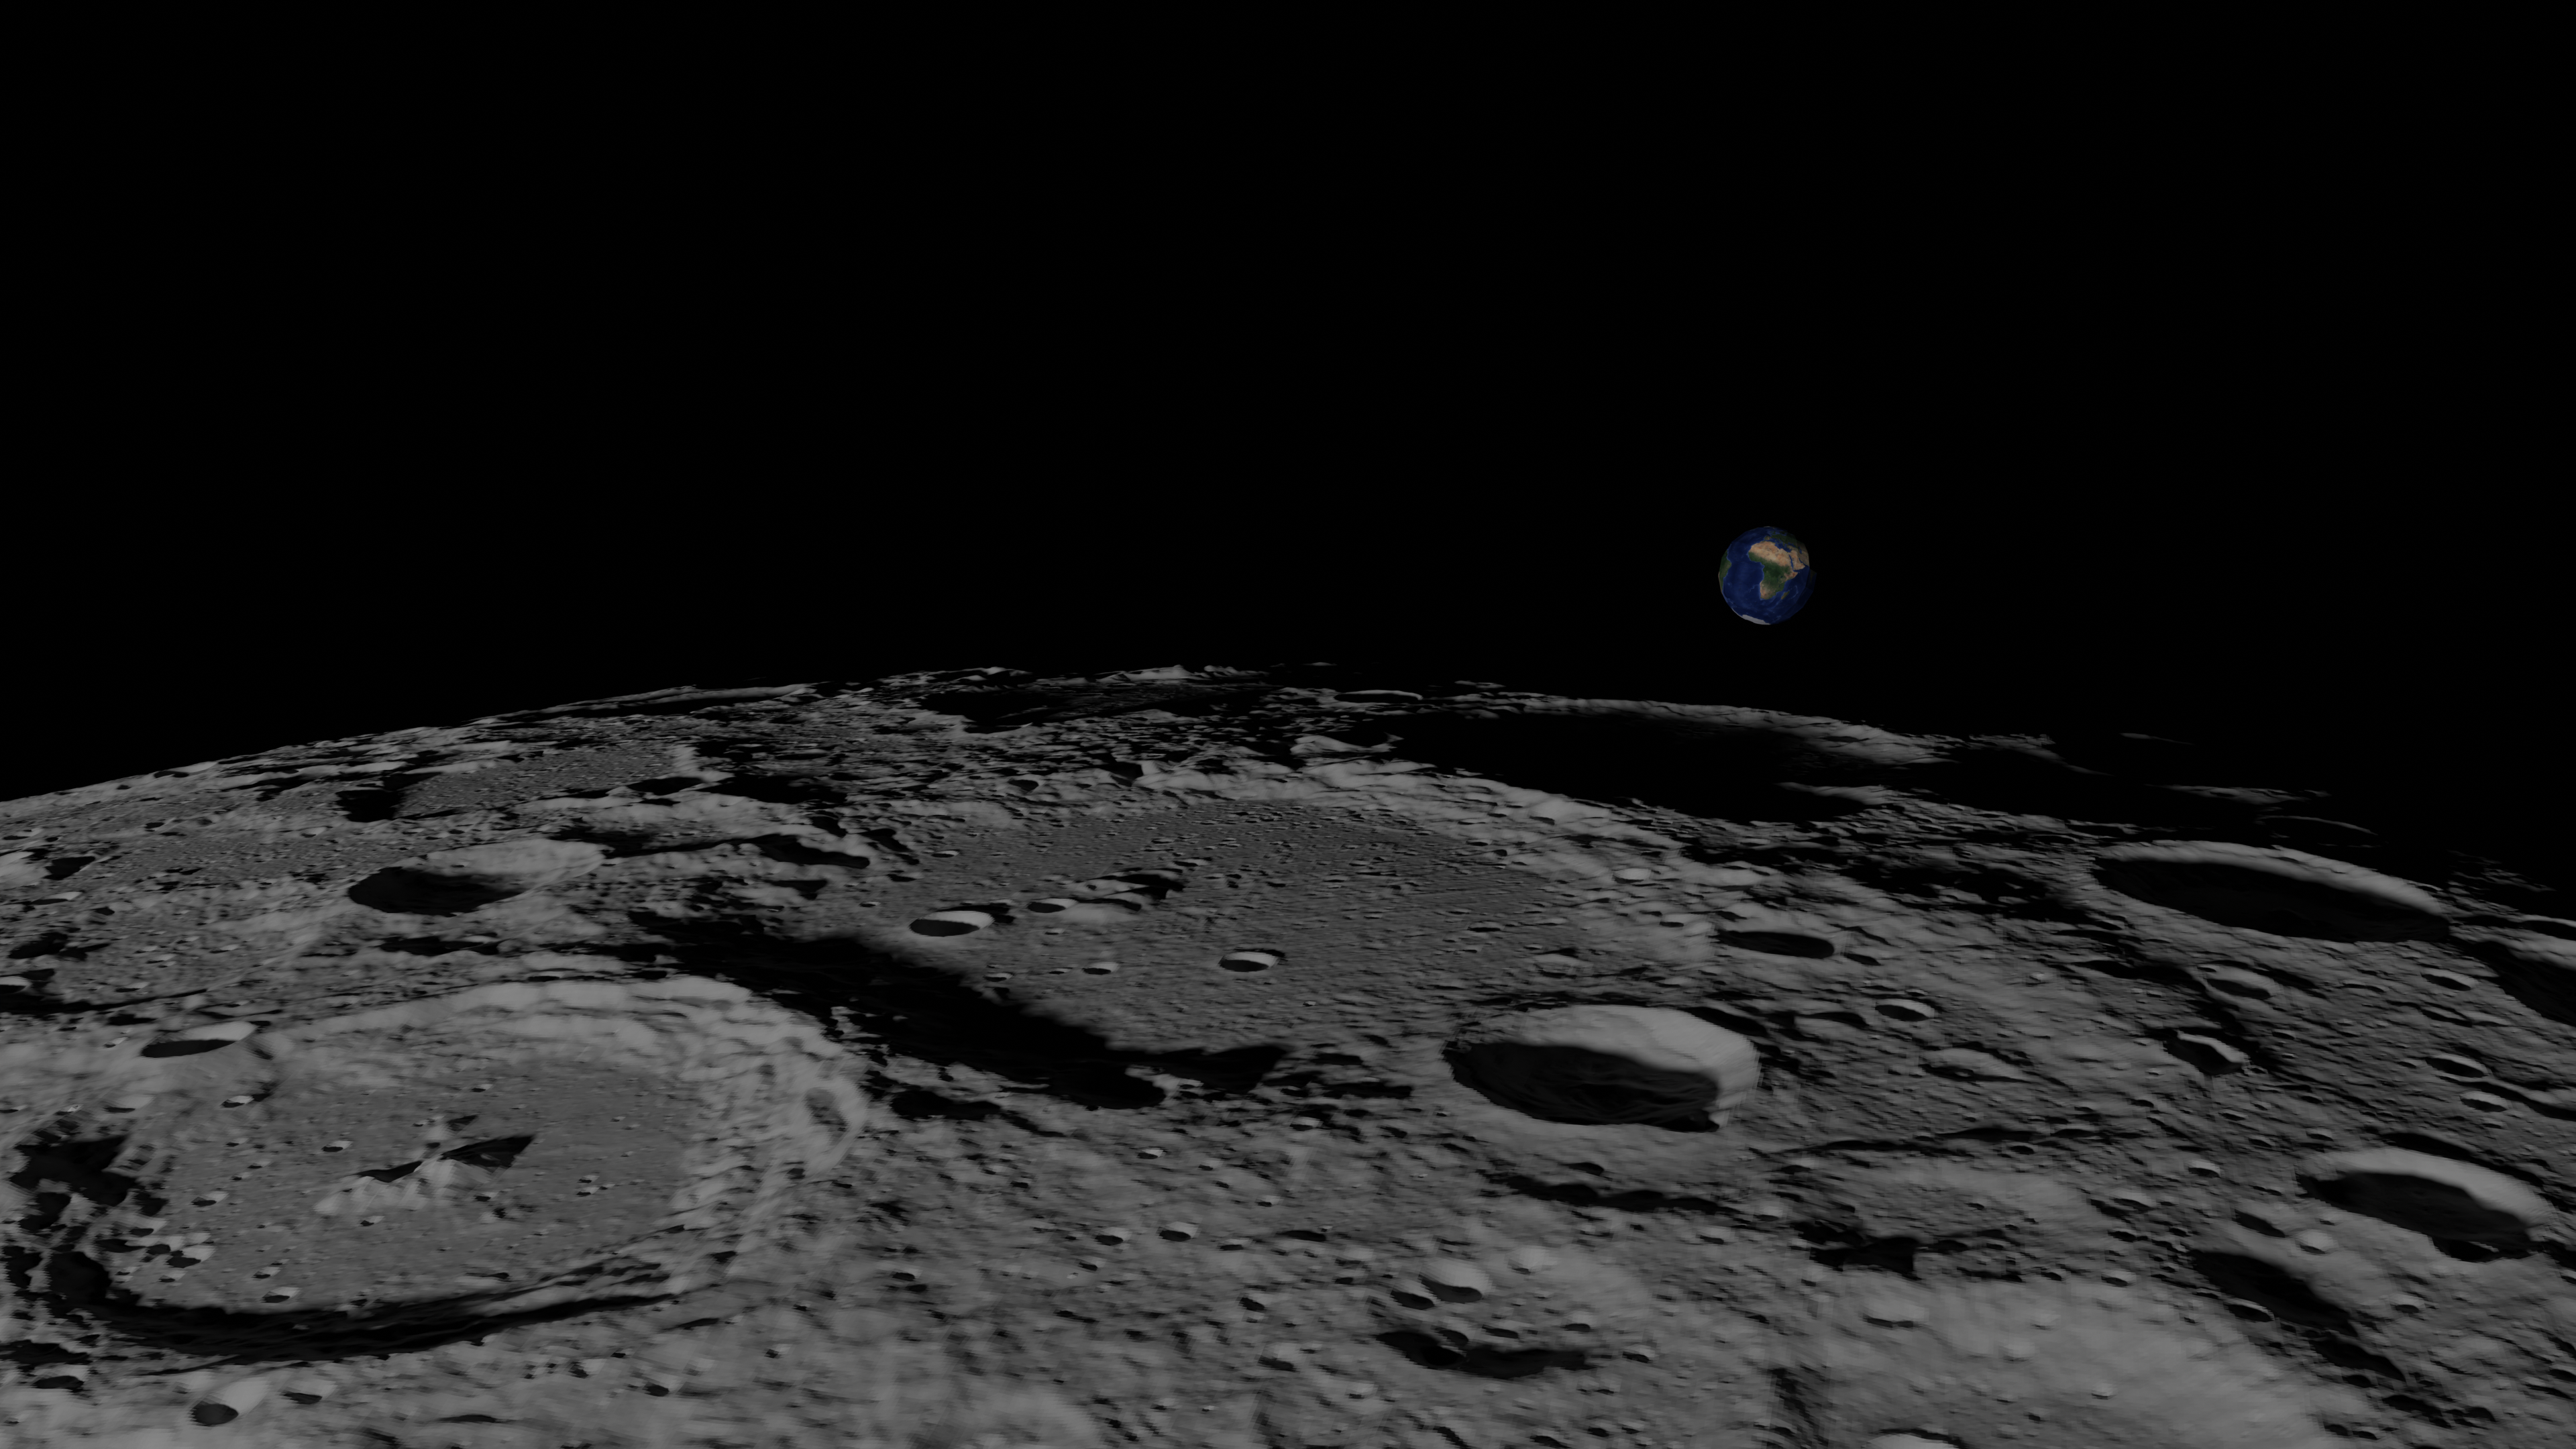
\includegraphics[width=0.8\textwidth]{./data/lro2_render.png}}
\end{figure}


The post on this picture mentions the name of the shot, M1145896768C. By googling it, we end up on \href{Link}{https://wms.lroc.asu.edu/lroc/view_lroc/LRO-L-LROC-3-CDR-V1.0/M1145896768CC} which tells us the sequence started on 2014-02-01 at 12:25:00.
One complication for this one, as the description page mentions, is that this was taken as the spacecraft was approaching the north pole. That means that the SLDEM2015 elevation data won't cover the visible area. 
All is not lost however as there is elevation data available around the poles.

Data can be downloaded \href{https://astrogeology.usgs.gov/search/details/Moon/LRO/LOLA/Lunar_LRO_LOLA_Global_LDEM_118m_Mar2014/cub}{here}.
This time, UV coordinates are not latlon but a \href{https://en.wikipedia.org/wiki/Stereographic_projection}{stereographic projection} onto the plane at the north pole.\\ 



The comparison is visible in fig \ref{img:lro2_diffs}. Again, differences in shadows between the rendered version and the original can be observed. The orientation of the moon is also slightly off. Compensating with the same tweak rotation as in the first picture helps a bit but the difference is still very noticeable.



\section{Reproducing this work}

All the data sources used are available online.

The python code is available \href{Link}{https://github.com/unjambonakap/chdrft/tree/master/sim}. This is a part of a monorepo (basically my programming/ folder).

Notebooks in \detokenize{./notebooks/{render_vtk,render_blender,moon_dem}} are the orchestrating points of this work.

\section{Wrap up}

All of this has needed a fair amount of time between getting familiar with software I knew nothing about, tooling up multiple times on different technos and over-abstracting to have a sort-of-reproducible work.
Pretty cool what you can do using data freely available on the internet!
I'm also downscaling the DEM data too much to load the mesh in Blender, there's still work here to get a better looking picture.

\bibliography{test.bib}{}
\bibliographystyle{plain}

\end{document}
